\documentclass{article}

%Packages

\usepackage[utf8]{inputenc}

\usepackage[parfill]{parskip}

\usepackage[colorlinks=true,urlcolor=codeblue]{hyperref}

\usepackage{graphicx}

%Document

\title{Software Sustainability - King's workshop exercises}

\author{Martin Chapman}

\date{Wednesday 2nd February 2022}

\begin{document}

\definecolor{bg}{rgb}{0.95,0.95,0.95}
\definecolor{codeblue}{rgb}{0,0.3,0.6}

\maketitle

\section{Prerequisites}

The below material assumes that the software sustainability course has been completed (\href{https://www.youtube.com/playlist?list=PLxyHJ\_wep1\_DPbvtFl\_-EGyoz2pVt-n1\_}{https://www.youtube.com/playlist?list=PLxyHJ\_wep1\_DPbvtFl\_-EGyoz2pVt-n1\_}), and that Python 3, Node.js, Git, Docker and Docker Compose are all installed.

\section{Background}

\begin{center}
    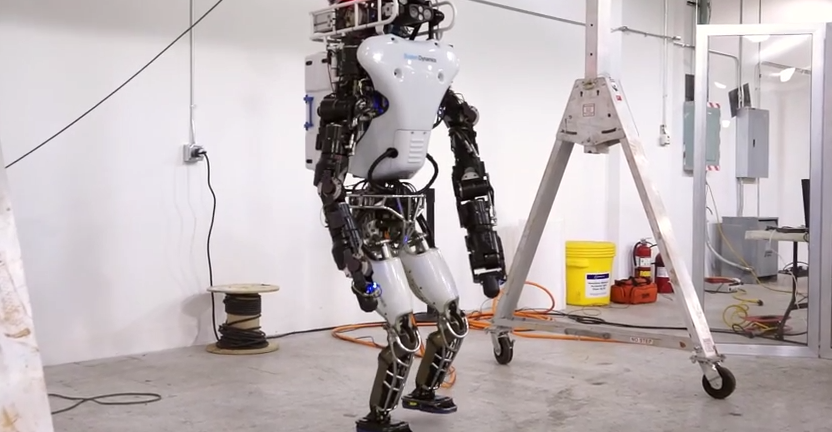
\includegraphics[height=5cm]{robot.png}
\end{center}

We are going to write a piece of code that simulates the movement of a robot in a 2D space from its starting position to a goal position, which is provided by a user. 

The robot being modelled is intelligent enough to know the direction it needs to move in to reach the target position, and this should be captured in the code.
For example, before each move the robot always starts at position $(0, 0)$ (an $X$ coordinate and a $Y$ coordinate, respectively) in the space, so if given a goal position of $(3, 3)$ it knows it needs to increase both its $X$ and $Y$ position until it arrives at the desired position (i.e. walk diagonally forward).

Once the simulated robot has reached its target position, our code should report the path it took to get there.
As such, the simulation allows us to evaluate the robot's AI.

We should also be able to probe for the robot's position at any time.

\subsection{Example}

\begin{enumerate}

    \item A user enters a goal position of $(3, 3)$. The robot is at position $(0, 0)$.

    \item The robot moves to position $(1, 1)$.

    \item The robot moves to position $(2, 2)$.

    \item The robot moves to position $(3, 3)$, which is the target position.

    \item The robot's path was $(1, 1)$, $(2, 2)$ $(3, 3)$, so this is reported back to the user.

\end{enumerate}

\begin{center}
  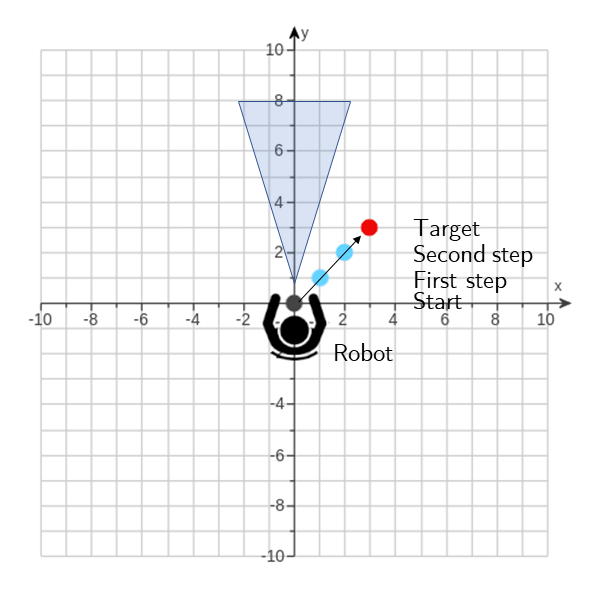
\includegraphics[height=5cm]{movement.png}
\end{center}

\section{Session 1 (10.10 - 10.50) - Coding practice}

Realise the simulation model described in Python code, adhering to the principles of coding practice discussed in the course.

Your code should accept a target position as input, simulate the movement of the robot towards that position, and report on the path the robot took to reach it.

\section{Session 2 (11.00 - 11.50) - Version control}

Make a version of your software, and push it to a remote repository on King's Github (\href{https://github.kcl.ac.uk/}{github.kcl.ac.uk}).
Call this repository `robot'.

You will need to log in with your k-number and password, if you have not done so before.

\textit{Public Github (\href{https://github.com}{github.com}), should
also work for this task, but should only be used as a backup.}

Additional versions should be made at appropriate points while completing the remaining tasks.

\section{Session 3 (12.00 - 12.50) - Testing}

Write three tests to ensure the following:

\begin{enumerate}

    \item The robot can move three steps down (backwards).

    \item The robot can move a large amount to the left (e.g. 10,000 steps).

    \item The robot is \textbf{not} still at position 0, when asked to move to position $(3, 3)$.

\end{enumerate}

Modify your program such that these tests pass, if needed.

You are welcome to add additional tests also.

\section{Session 4 (14.00 - 14.50) - Services}

The supporting material for this session are available at
\href{https://github.com/martinteaching/sustainability}{github.com/martinteaching/sustainability}.

Wrap your Python robot simulation model in a server and run it.

Move the request for target position to a Javascript client, which, once acquired, sends this information to the server, waits for the robot simulation to complete, and then prints the path of the robot for the user.

\section{Session 5 (15.00 - 15.50) - Docker}

Dockerise your program -- using a Dockerfile and Docker Compose -- allowing the Python server to run in a container, and the Javascript client to issue requests to it.

\section{Additional Tasks}

If you wish to expand on your solution, create a second Python service that encapsulates the logic required to place $N$ objects randomly in a 2D space, each with a coordinate. 
Every time your robot moves, the simulation code (contained in a service) should call this second service to determine whether the robot has hit an object (i.e. the robot's current coordinates are the same as the coordinates of one of the objects).
The total number of collisions should be recorded and reported back to the user along with the robot's path.

Under this setup, the client calls a service (robot), which in turn calls a second service (object) as a part of its operation before reporting the results back to the client.

\section{Assessment}

Attendees at the workshop will be given time to review and start these exercises individually, and will then be asked to complete them fully with each other in an online collaborative environment.

Sufficient engagement with these collaborative sessions will result in a `pass' mark for the workshop.

\end{document}
